% Fig. 1 — montagem e esquema de medição (vista de cima, fora de escala)
\resizebox{\columnwidth}{!}{%
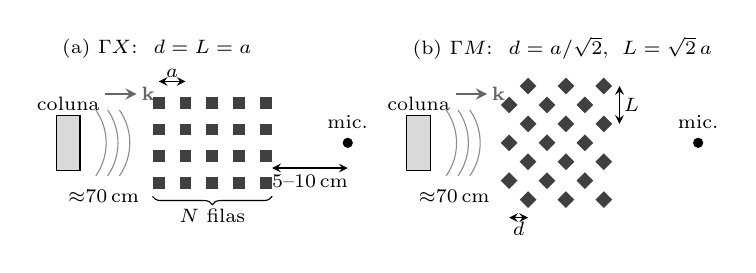
\begin{tikzpicture}[x=1cm,y=1cm,
    tij/.style={fill=black!75,draw=none},
    lbl/.style={font=\scriptsize},
    cota/.style={<->,>=stealth,thin}]
  \def\a{0.34}
  \pgfmathsetmacro{\d}{\a/sqrt(2)}
  \pgfmathsetmacro{\L}{\a*sqrt(2)}
  % coluna de som + frentes de onda (comum aos dois painéis)
  \newcommand{\fonte}{%
    \draw[fill=black!15] (0,-0.35) rectangle (0.3,0.35);
    \foreach \r in {0.5,0.65,0.8}
      \draw[black!45,thin] (\r,-0.42) arc[start angle=-35,end angle=35,radius=0.73];
    \draw[->,>=stealth,thick,black!60] (0.62,0.62) -- (1.02,0.62) node[right=-2pt,lbl] {$\mathbf k$};
    \node[lbl] at (0.6,-0.68) {$\approx$70\,cm};
    \node[lbl] at (0.15,0.5) {coluna};
    \fill (3.7,0) circle (0.065);
    \node[lbl] at (3.7,0.27) {mic.};}
  % ---------------------------------------------------------------- (a) ΓX
  \begin{scope}
    \node[lbl,anchor=west] at (-0.05,1.2) {(a) $\Gamma X$:\; $d=L=a$};
    \fonte
    \foreach \i in {0,...,4}
      \foreach \j in {-1.5,-0.5,0.5,1.5}
        \fill[tij] ({1.3+\i*\a-0.075},{\j*\a-0.075}) rectangle ++(0.15,0.15);
    \draw[cota] (1.3,0.78) -- (1.3+\a,0.78) node[midway,above=-2pt,lbl] {$a$};
    \draw[decorate,decoration={brace,amplitude=3pt,mirror}] (1.22,-0.68) -- ({1.3+4*\a+0.08},-0.68)
      node[midway,below=1pt,lbl] {$N$ filas};
    \draw[cota] ({1.3+4*\a+0.08},-0.32) -- (3.7,-0.32) node[midway,below=-1pt,lbl] {5--10\,cm};
  \end{scope}
  % ---------------------------------------------------------------- (b) ΓM
  \begin{scope}[xshift=4.45cm]
    \node[lbl,anchor=west] at (-0.05,1.2) {(b) $\Gamma M$:\; $d=a/\sqrt2$,\; $L=\sqrt2\,a$};
    \fonte
    \foreach \i in {0,...,5} {
      \pgfmathtruncatemacro{\paridade}{mod(\i,2)}
      \ifnum\paridade=0
        \foreach \j in {-1,0,1}
          \fill[tij,rotate around={45:({1.3+\i*\d},{\j*\L})}] ({1.3+\i*\d-0.075},{\j*\L-0.075}) rectangle ++(0.15,0.15);
      \else
        \foreach \j in {-1.5,-0.5,0.5,1.5}
          \fill[tij,rotate around={45:({1.3+\i*\d},{\j*\L})}] ({1.3+\i*\d-0.075},{\j*\L-0.075}) rectangle ++(0.15,0.15);
      \fi
    }
    \draw[cota] (1.3,-0.95) -- ({1.3+\d},-0.95) node[midway,below=-2pt,lbl] {$d$};
    \draw[cota] ({1.3+5*\d+0.2},{0.5*\L}) -- ({1.3+5*\d+0.2},{1.5*\L}) node[midway,right=-2pt,lbl] {$L$};
  \end{scope}
\end{tikzpicture}}
